\def\regenfigs{0}
\documentclass[anonymous,sigconf,9pt]{acmart}

\usepackage{microtype}
\if\regenfigs1
\usepackage{tikz,pgfplots}
\usetikzlibrary{arrows.meta}
\usepgfplotslibrary{groupplots}
\usepgfplotslibrary{external}
\usepgfplotslibrary{colorbrewer}
\pgfplotsset{cycle list/Set1}
\usepgfplotslibrary{fillbetween}
\pgfplotsset{compat=1.18}
\pgfplotsset{
    tick align=outside,
    tick pos=left,
    xmajorgrids,
    x grid style={white},
    ymajorgrids,
    y grid style={white},
    axis line style={white},
    axis background/.style={fill=white!89.803921568627459!black},
    legend style={draw=none, fill=none},
    legend cell align=left,
}
\pgfkeys{/pgf/number format/.cd, 1000 sep={\,}}

\pgfplotsset{
    log x ticks with fixed point/.style={
        xticklabel={
            \pgfkeys{/pgf/fpu=true}
            \pgfmathparse{2^\tick}
            \pgfmathprintnumber[fixed relative, precision=4]{\pgfmathresult}
            \pgfkeys{/pgf/fpu=false}
        }
    },
    log10 x ticks with fixed point/.style={
        xticklabel={
            \pgfkeys{/pgf/fpu=true}
            \pgfmathparse{10^\tick}%
            \pgfmathprintnumber[fixed relative, precision=3]{\pgfmathresult}
            \pgfkeys{/pgf/fpu=false}
        }
    },
    log y ticks with fixed point/.style={
        yticklabel={
            \pgfkeys{/pgf/fpu=true}
            \pgfmathparse{2^\tick}%
            \pgfmathprintnumber[fixed relative, precision=4]{\pgfmathresult}
            \pgfkeys{/pgf/fpu=false}
        }
    }
}
\fi

\begin{document}

\definecolor{alps}{RGB}{35,139,69}
\definecolor{aurora}{RGB}{107,174,214}
\definecolor{frontier}{RGB}{239,59,44}
\definecolor{eos}{RGB}{253,141,60}
\begin{figure*}[tbp]
\if\regenfigs1
\begin{tikzpicture}[overlay=false,>=latex]
    \begin{groupplot}[
            /tikz/overlay=false,
            /tikz/thick,
            group style={
                group size=3 by 1,
                vertical sep=0.2cm,
                horizontal sep=0.9cm,
                xlabels at=edge bottom,
                ylabels at=edge left,
                xticklabels at=edge bottom,
            },
            width=\linewidth/2,
            ylabel near ticks,
            xlabel={\# GPU nodes},
            xmode=log,
            ymode=log,
            log basis x=10,
            xmin=0.5, xmax=3500,
            %log10 x ticks with fixed point,
            clip=false,
            title style={yshift=-0.5cm, xshift=-2.1cm,anchor=west},
            %ylabel style={xshift=1.2cm},
            ylabel={timesteps/s},
            height=2.1in,
            width=2.5in,
        ]
            
            \nextgroupplot[
                ymin=2, ymax=5050,
                legend style={at={(0.7,0.3)},anchor=east},
                legend columns=1,
                title={a) LJ},
            ]
            
            \addplot+[mark=square*,alps]  table[y expr={\thisrowno{2}*0.8192}] {results_alps/lj-8M-4gpus.txt};
            \addplot+[mark=square*,alps]  table[y expr={\thisrowno{2}*1.05}] {results_alps/lj-1B-4gpus.txt};
            \addplot+[mark=square*,alps]  table[y expr={\thisrowno{2}*1.342}] {results_alps/lj-128B-4gpus.txt};

            \addplot+[mark=*,eos]  table[y expr={\thisrowno{2}*0.8192}] {results_eos/lj_8M.txt};
            \addplot+[mark=*,eos]  table[y expr={\thisrowno{2}*1.05}] {results_eos/lj_1B.txt};
            \addplot+[mark=*,eos]  table[y expr={\thisrowno{2}*1.342}] {results_eos/lj_128B.txt};
            
            \draw (axis cs:1,400) node[anchor=north] {\(10^7\)};
            \draw (axis cs:2,8) node[anchor=135] {\(10^9\) atoms};
            \draw (axis cs:256,6) node[anchor=north] {\(10^{11}\)};
            
            \nextgroupplot[
                ymin=2, ymax=205,
                legend style={at={(0.5,1.0)},anchor=south},
                legend columns=9,
                title={b) ReaxFF},
            ]
            \addplot+[mark=square*,alps]  table[y expr={\thisrowno{2}*0.9339}] {results_alps/reaxff-1M-4gpus.txt};
            \addlegendentry{Alps (4\(\times\)GH200)};
            \addplot+[mark=*,eos]  table[y expr={\thisrowno{2}*0.9339}] {results_eos/hns_1M.txt};
            \addlegendentry{Eos (4\(\times\)H100)};
            
            \addplot+[mark=square*,alps]  table[y expr={\thisrowno{2}*1.195}] {results_alps/reaxff-128M-4gpus.txt};
            \addplot+[mark=square*,alps]  table[y expr={\thisrowno{2}*1.53}] {results_alps/reaxff-16B-4gpus.txt};
            \addplot+[mark=*,eos]  table[y expr={\thisrowno{2}*1.195}] {results_eos/hns_128M.txt};
            
            \draw (axis cs:1,28) node[anchor=north] {\(10^6\)};
            \draw (axis cs:8,3) node[anchor=west] {\(10^8\)};
            \draw (axis cs:1024,4) node[anchor=south] {\(10^{10}\)};
            
            \nextgroupplot[
                ymin=0.11, ymax=2050,
                legend style={at={(1.0,0.2)},anchor=east},
                legend columns=1,
                title={c) SNAP},
            ]
            
            \addplot+[mark=square*,alps]  table[y expr={\thisrowno{2}*1.024}] {results_alps/snap-1M-4gpus.txt};
            \addplot+[mark=square*,alps]  table[y expr={\thisrowno{2}*1.31}] {results_alps/snap-128M-4gpus.txt};
            \addplot+[mark=square*,alps]  table[y expr={\thisrowno{2}*1.68}] {results_alps/snap-16B-4gpus.txt};
            
            \addplot+[mark=*,eos]  table[y expr={\thisrowno{2}*1.024}] {results_eos/snap_1M.txt};
            \addplot+[mark=*,eos]  table[y expr={\thisrowno{2}*1.31}] {results_eos/snap_128M.txt};
            \addplot+[mark=*,eos]  table[y expr={\thisrowno{2}*1.68}] {results_eos/snap_16B.txt};
            
            \draw (axis cs:1,20) node[anchor=north] {\(10^6\)};
            \draw (axis cs:2,0.25) node[anchor=west] {\(10^8\)};
            \draw (axis cs:128,0.2) node[anchor=west] {\(10^{10}\)};
    \end{groupplot}
\end{tikzpicture}
\else
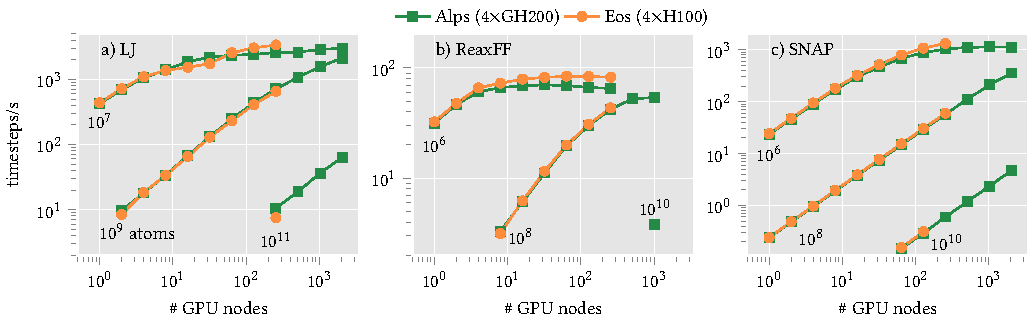
\includegraphics{generated-figures/paper-figure7.pdf}
\fi
\caption{Strong scaling results for LAMMPS on NVIDIA Eos and CSCS Alps, comparing H100 to GH200 performance across all benchmarks. The data from Alps is identical to the data from figure~\ref{fig:strongscaling}.}\label{fig:eosalps}
\end{figure*}

\end{document}
